
\begin{appendices}

	
	
	\section{{Overview of Business Groups in Tehran Stock Exchange}} \label{BGDef}
	There is no difference between emerging markets (such as  Chile, India, Indonesia, South Korea, Pakistan, and many more) and developed ones (like Italy and Sweden); business groups present everywhere. However, group-affiliated firms are relatively large and economically important in emerging markets. 
	These groups principally consist of legally independent firms grouped by persistent formal (e.g., equity) and informal (e.g., family) links.(\cite{khanna2007business}) 
	There is a complex ownership network in TSE as an emerging market. 
	This complicated ownership creates a vast number of business groups in which an ultimate owner controls them through a multi-layer of ownership. (\cite{FirmInterlock})
	
	
	
	
	The reason for many of these business groups back to the 1979 Iran revolution. After the revolution, due to social sentiment, critical sectors of the economy nationalized, and their ownership transferred to the government or other pseudo-government foundations. Also,
	some other groups of firms in heavy industries were established and controlled by the Industrial Development and Renovation Organization (IDRO) during the 1960s and 1970s. (IDRO was a state-owned holding company for investing in capital-intensive industries) 
	
	The business groups are formed from mentioned ancestors due to two related forces; A multi-phased privatization by the state and the development of the domestic stock market. In the first wave of privatization, more than 300 companies were fully or partially privatized. In the second one, approximately  \$150 billion ownership of State-Owned Enterprises (SOEs) and assets were transferred.  
	Pension funds, military institutions, cultural and religious foundations, and revolutionary foundations (pseudo-government groups) primary customers in the second wave of privatization. These waves of privatization transferred control of hundreds of SOEs to semi-governmental groups and were the main driver of the formation of business groups in Iran. In addition, the developing stock market from the early 2000s intensifies this effect. The government tried to develop the stock market as a tool for better privatization. 
	(\cite{Aliabadi2022})
	
	In conclusion, the multiple waves of privatization with the development of the stock market changed ownership structure in pre-revolutionary holding companies and post-revolutionary foundations and create large business groups that govern primary  industries.
	
	

%			\begin{figure}[htbp]
%				\caption{}
%				\label{sameIndustryinBG}
%				\centering
%				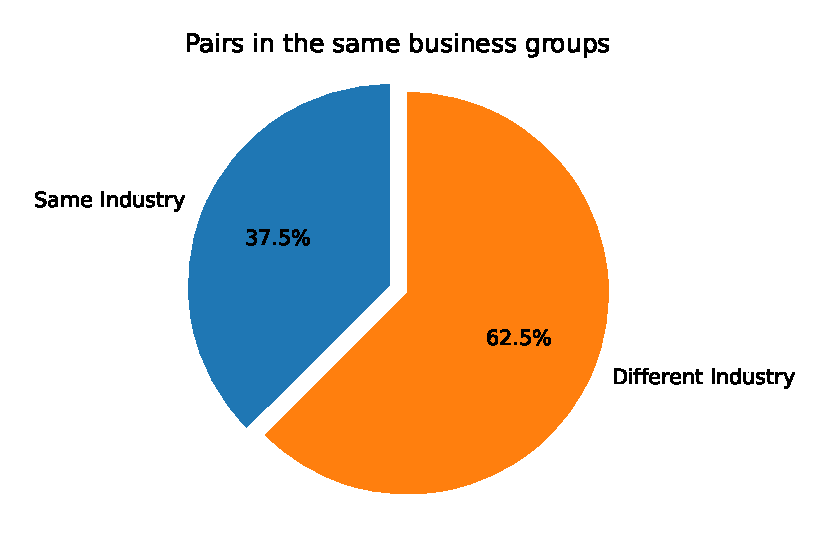
\includegraphics[width=0.48\linewidth]{Output/sameIndustryinBG.eps}
%				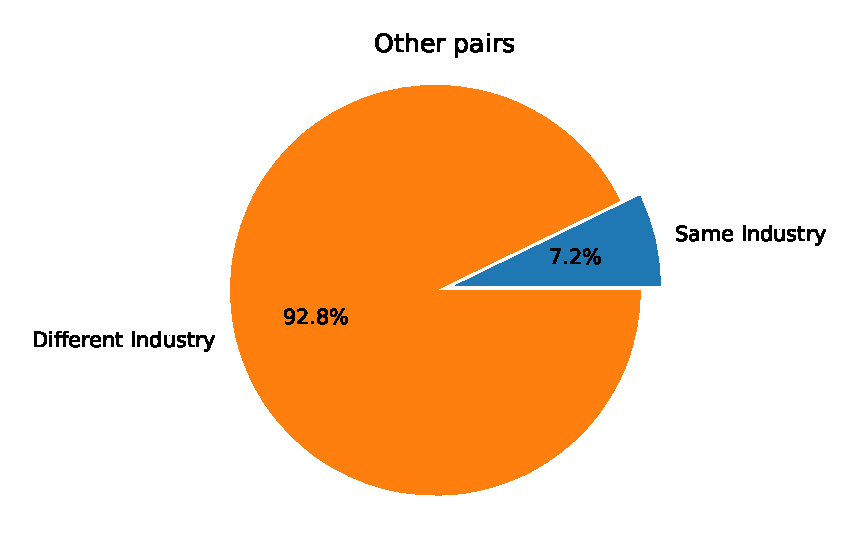
\includegraphics[width=0.48\linewidth]{Output/sameIndustryNoinBG.eps}
%			\end{figure}
%		
%			\begin{figure}[htbp]
%				\caption{}
%				\label{BGSummary}
%				\centering
%				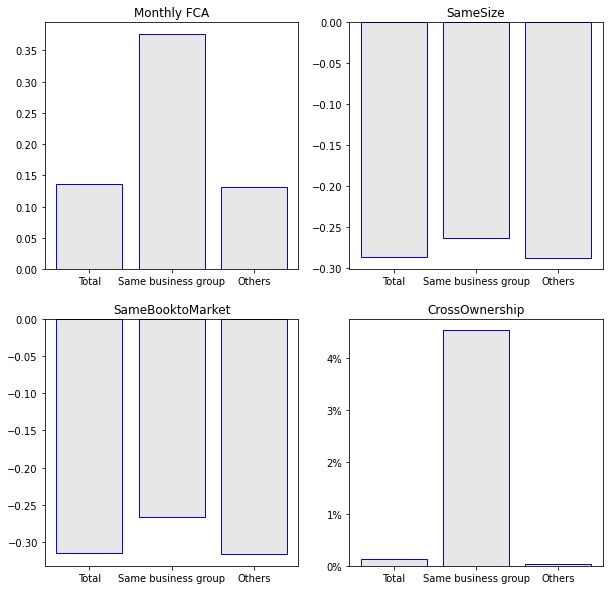
\includegraphics[width=0.85\linewidth]{Output/BGSummary.eps}
%			\end{figure}
%	
	
	
	\FloatBarrier


	\section{{Modified Anton's measure}}
	\label{ModifiedMeasure}
We reformulate mentioned Anton's measure in table \ref{maasurmentsSummary}. This factor measure common ownership as the total value of
stock held by the F common-holders of the two stocks, scaled by the total market capitalization of the two stocks

		\begin{equation}
			\text{Overlap}_{Sum}(i, j) = \frac{\sum_{f = 1}^{F} (S^f_{i,t}P_{i,t}+S^f_{j,t}P_{j,t})}{S_{i,t}P{i,t} + S_{j,t}P{j,t}}
			\label{Sum}
		\end{equation}
where $ S^f_{i,t}$ is the number of shares held by owner f
at time t trading at price $ P{i,t} $ with total shares outstanding of $ S_{i,t} $, and similarly for stock j. 
As shown in equation \ref{Sum}, this measure neglects different distributions of common owners and represents the percent of joint-held market capitalization from the total market capitalization of the two stocks.

We re-weight this formula to capture the difference between ownership distributions. Our proposed measures are shown in equations \ref{sqrt} and \ref{Quadratic}, where all variables are as the same as Anton's measure. Both modified measures represent the number of block-holders with equal-percent ownership. In other words, if for a pair of stocks with n mutual owners, all owners have even shares of each firm's market cap, the proposed indices equals to the number of holders.\footnote{Each holder owns $ 1/n $ of each firm ,firm's market cap is $ \alpha_1 $ and $ \alpha_2 $, so for each holder of firms we have $ S^f_{i,t}P_{i,t} = \alpha_i/n $\\
		$
		[  \frac{\sum_{f=1}^{n} \sqrt{\alpha_1/n}+\sum_{f=1}^{n} \sqrt{\alpha_2/n}}{\sqrt{\alpha_1} + \sqrt{\alpha_2}}]^2 
		= [\frac{\sqrt{n}(\sqrt{\alpha_1} +\sqrt{\alpha_2 })}{\sqrt{\alpha_1} + \sqrt{\alpha_2}}]^2 = n $
		\\
		$
		[\frac{\sum_{f=1}^{n} {(\alpha_1/n)^2}+\sum_{f=1}^{n} {(\alpha_2/n)^2}}{\alpha_1^2 +{\alpha_2}^2}]^{-1} = [\frac{{\alpha_1^2 + \alpha_2^2 }}{n(\alpha_1^2 + \alpha_2^2)}]^{-1} = n
		$} There are some numeric examples for a better comparison. 

		\begin{equation}
			\text{Overlap}_{Sqrt}(i, j) =  [\frac{\sum_{f =1}^{F}(\sqrt{S^f_{i,t}P_{i,t}}+\sqrt{S^f_{j,t}P_{j,t}})}{\sqrt{S_{i,t}P{i,t}} + \sqrt{S_{j,t}P{j,t}}}]^2 
			\label{sqrt}
		\end{equation}
		
		\begin{equation}
			\text{Overlap}_{Quadratic}(i, j) =  [{\frac{\sum_{f = 1}^{F}[(S^f_{i,t}P_{i,t})^2+(S^f_{j,t}P_{j,t})^2]}{(S_{i,t}P{i,t})^2 + (S_{j,t}P{j,t})^2}}]^{-1}
			\label{Quadratic}
		\end{equation}


For the first example, two firms (X and Y) have one common owner who has $ \alpha $ and $ \beta $ from each market capitalization, respectively (illustrated in figure \ref{gExample1}).  
For better illustration, assume that the sum of holders' ownership equals to 100 percent ($ \alpha + \beta  = 100$), and two firms' market caps have equal amounts. 
				\begin{figure}[htbp]
					\centering
					\caption{{ Numeric example 1} }
					\label{gExample1}
					\resizebox{0.65\textwidth}{!}{
										\begin{tikzpicture}[node distance=1cm]
											
											\node (Firm) [startstop3] {\tiny Firm X};
											\node (Firm2) [startstop3,right of = Firm  , xshift=-5.5cm ] {\tiny Firm Y};
											\node (Owner) [startstop3,right of = Firm , yshift=1cm , xshift=-3.25cm ] {\tiny Common owner };
											
											
											\draw[arrow] (Owner) -- node[sloped, anchor=center, above] {\tiny $ \alpha $} (Firm) ;
											
											\draw[arrow] (Owner) -- node[sloped, anchor=center, above] {\tiny $ \beta $} (Firm2) ;
											%
											%\node() at (3,0)
											%    {$ \alpha + \beta = 100 $}; 
										\end{tikzpicture}
									}
									\end{figure}		
We  calculate common ownership measures based on equations \ref{Sum} (Sum), \ref{sqrt} (SQRT), and \ref{Quadratic} (Quadratic) for different ownership distributions. Figure \ref{example1Results}  reports calculations results. As we expected, Anton's measure is constant at a fixed level of aggregated common ownership, but SQRT and Quadratic vary from concentrated to dispersed ownership.  Concentrated ownership (50-50) has a greater common ownership measure than dispersed (10-90).
				
				\begin{figure}[htbp]
					\caption{ {Comparison of three measures for common ownership}}
					\label{example1Results}
					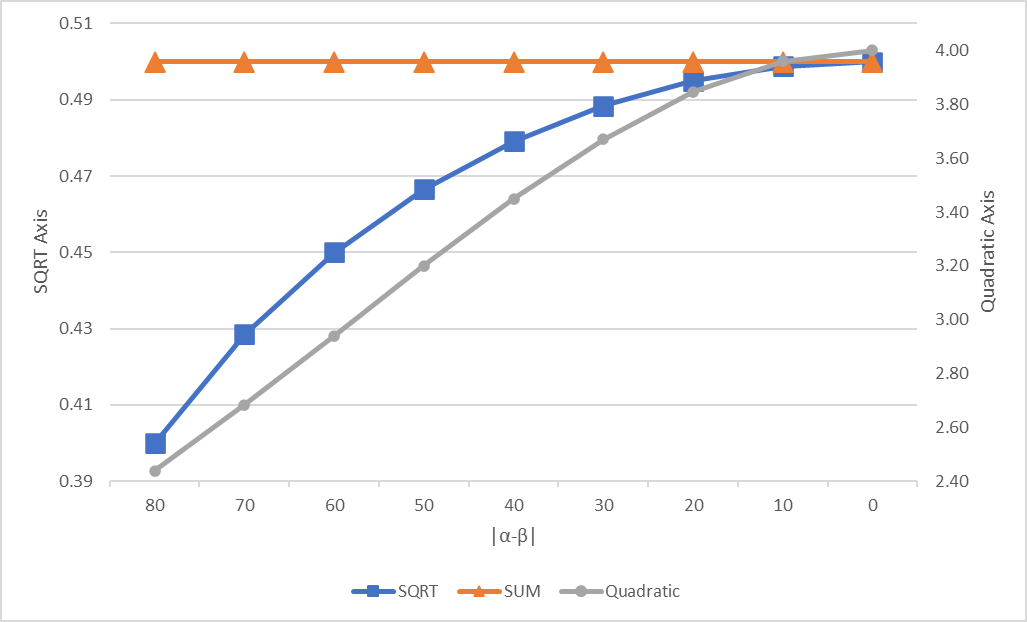
\includegraphics[width=0.47\linewidth]{Elements/1.png}
					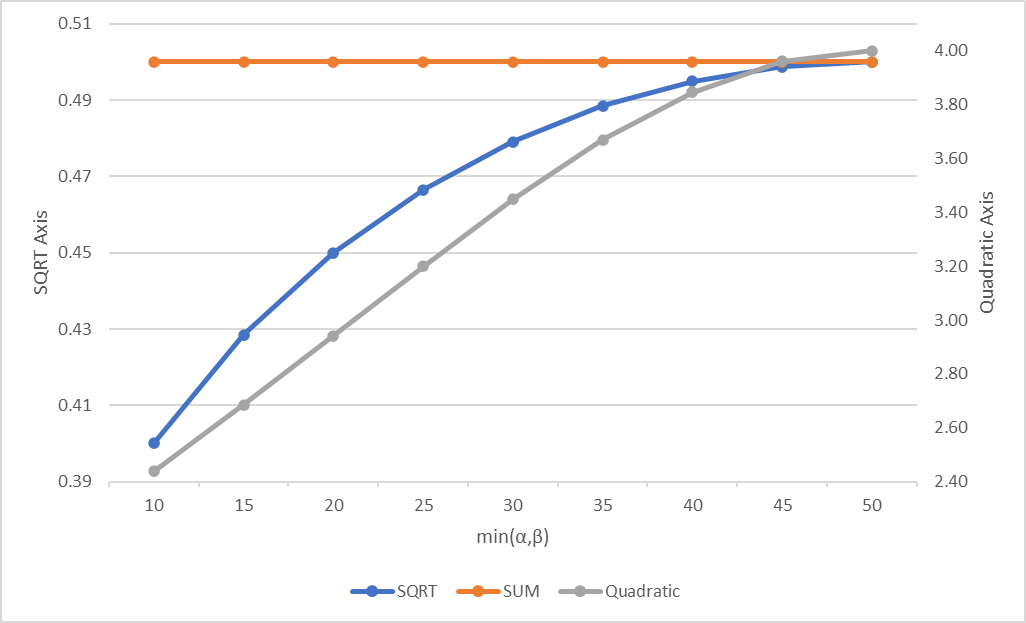
\includegraphics[width=0.47\linewidth]{Elements/2.png}
				\end{figure}

For the second example, assume that there are three common owners for the two mentioned firms. First holder's ownership from firm X and Y are respectively $\alpha_1$ and $\beta_1$. It is similar for other holders (illustrated in figure \ref{gExample2}). As before, the firm's market cap is equal. We calculate measures for concentrated or disparate ownerships, and ownerships that are less than the sum of the market caps. Table \ref{Example2} reports calculation results. For ownerships that consist of total market cap,  results are consistent with the first example. Although, when total ownership decreases, the Quadratic measure denotes unrealistic numbers. We conclude that our Quadratic measure is not suitable for lower levels of common ownership.
				
				\begin{figure}[htbp]  \centering
					\caption{ Numeric example 2}
					\label{gExample2}
					\centering
					\begin{tikzpicture}[node distance=1cm]
						
						
						\node (Firm) [startstop3] {\tiny Firm X};
						\node (Firm2) [startstop3,right of = Firm , yshift=0cm , xshift=-8cm ] {\tiny Firm Y};
						
						\node (Owner) [startstop3,above of = Firm , yshift=1.25cm , xshift=-3.5cm ] {\tiny Common owner 1 };
						
						
						\node (Owner2) [startstop3,right of = Firm , yshift= 0 , xshift=-4.5cm ] {\tiny Common owner 2 };
						
						\node (Owner3) [startstop3,below of = Firm , yshift=-1.25cm , xshift=-3.5cm ] {\tiny Common owner 3 };
						
						
						
						
						
						\draw [-latex] (Owner) to [bend right =0]  node[sloped, anchor=center, above] {\tiny $ \beta_1 $} (Firm2);
						
						\draw [-latex] (Owner) to [bend left =0]  node[sloped, anchor=center, above] {\tiny $ \alpha_1 $} (Firm);
						
						
						
						\draw [-latex] (Owner2) to [bend right =0]  node[sloped, anchor=center, below] {\tiny $ \beta_2 $} (Firm2);
						
						\draw [-latex] (Owner2) to [bend left =0]  node[sloped, anchor=center, below] {\tiny $ \alpha_2 $} (Firm);
						
						
						
						\draw [-latex] (Owner3) to [bend left =0]  node[sloped, anchor=center, below] {\tiny$ \beta_3 $} (Firm2);
						
						\draw [-latex] (Owner3) to [bend right =0]  node[sloped, anchor=center, below] {\tiny $ \alpha_3 $} (Firm);
						
						
						
					\end{tikzpicture}
				\end{figure}
			{\begin{table}[htbp]
							\centering
							\caption{ text}
							\label{Example2}
							\resizebox{1\textwidth}{!}
							{
								    \begin{tabular}{cccccccc}
    \hline\hline
        Ownership  & Type I & Type II & Type III & Type IV & Type V & Type VI & Type VII \\
          \hline
    $ \alpha_1 $    & 1/3 &20      &  10   & 20    & 10    & 5     & 1  \\
    $ \beta_1 $    & 1/3  & 10    & 10   & 20    & 10    & 5     & 1  \\
    $ \alpha_2 $    & 1/3  & 10    & 80    & 20    & 10    & 5     & 1 \\
    $ \beta_2 $    & 1/3  & 20    & 80    & 20    & 10    & 5     & 1  \\
    $ \alpha_3 $    & 1/3  & 70    & 10    & 20    & 10    & 5     & 1 \\
    $ \beta_3 $    & 1/3  & 70    & 10   & 20    & 10    & 5     & 1  \\
    \hline
    SQRT  & 3     &  2.56  & 2.33 & 1.8   & 0.9   & 0.45  & 0.09 \\
    SUM   & 1     & 1     & 1     & 0.6   & 0.3   & 0.15  & 0.03 \\
    Quadratic & 3     & 1.85  & 1.52  & 8.33  & 33.33 & 133.33 & 3333.33 \\
 
    \hline\hline
    \end{tabular}%
							}
					\end{table}}
				

A fundamental assumption in previous examples, is the equality of firms' market cap. In the last example, we relax this assumption. Table \ref{marketcap} reports calculated measures for fixed total ownership on different relative market cap ratios. We extend our analysis to higher market cap ratios and report our results in figures \ref{sqrtMarket} and \ref{sumMarket}. In this setting, the SQRT measure has a better variation compared to Anton's measure. 

				
	
					\begin{figure}[htbp]
							\centering
							\caption{ SQRT measure for fixed aggregate ownership on different relative market cap ratios}
							\label{sqrtMarket}
							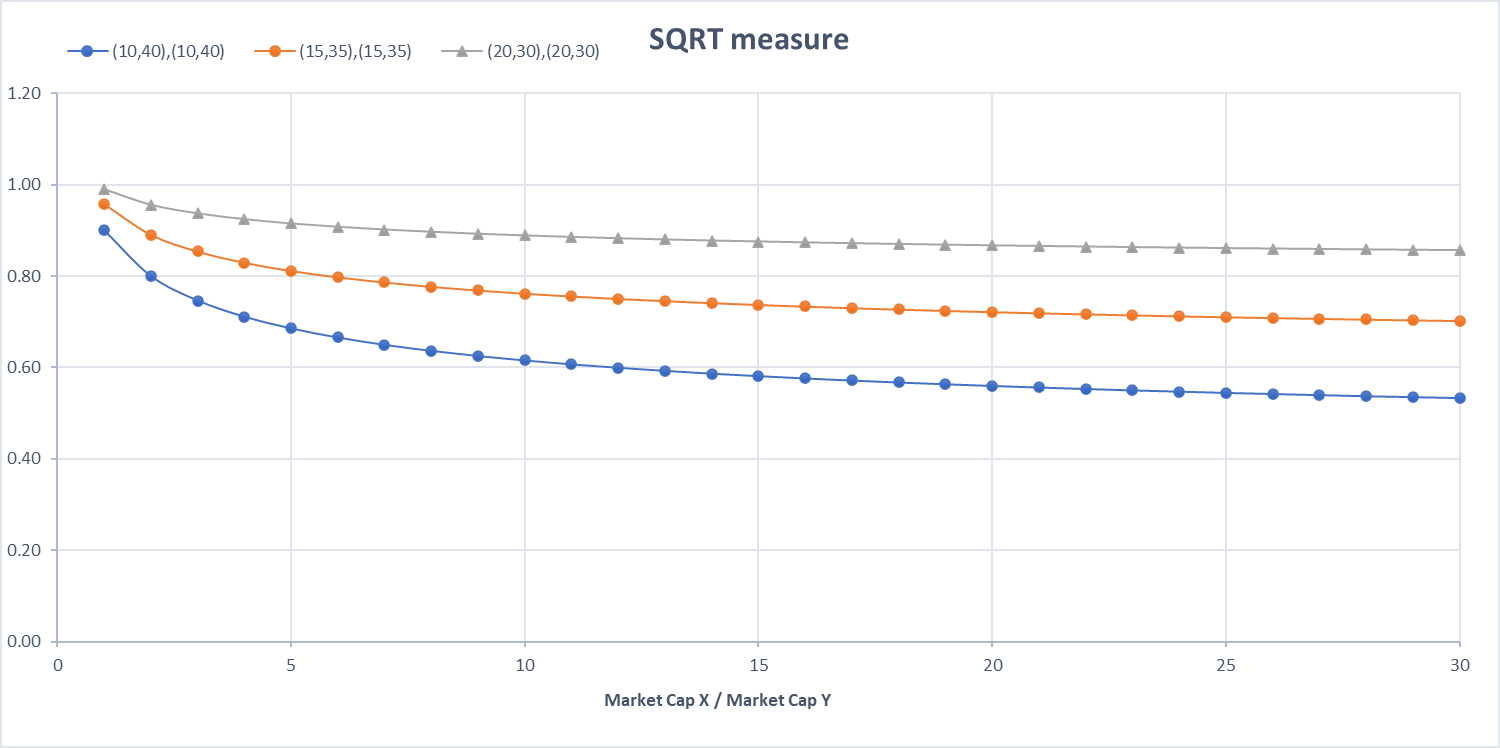
\includegraphics[width=0.85\linewidth]{Elements/3.png}
						\end{figure}
						\begin{figure}[htbp]
							\centering
							\caption{ Sum measure for fixed aggregate ownership on different relative market cap ratios}
							\label{sumMarket}
							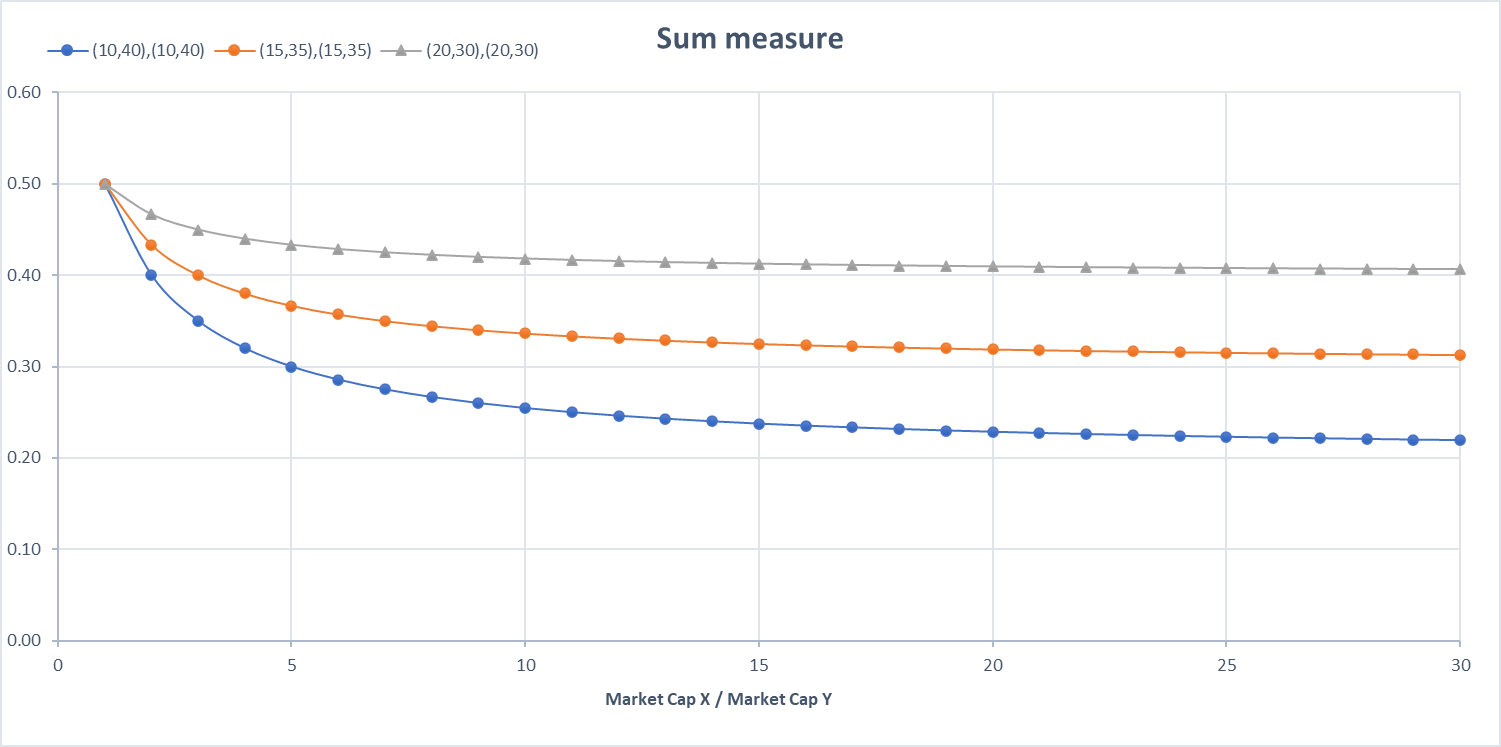
\includegraphics[width=0.85\linewidth]{Elements/4.png}
					\end{figure}
				\begin{table}[htbp]
							\centering
							\caption{text }
							\label{marketcap}
							\resizebox{0.9\textwidth}{!}
							{
								          \scriptsize
    \begin{tabular}{ccccccc}
    \hline\hline
  & \multicolumn{6}{c}{\tiny($ \alpha_1 $,$ \beta_1 $),($ \alpha_2 $,$ \beta_2 $) }\\ \cmidrule(lr){2-7}
               & \multicolumn{2}{c}{\tiny(10,40),(10,40)} & \multicolumn{2}{c}{\tiny(15,35),(15,35)} & \multicolumn{2}{c}{\tiny(20,30),(20,30)} \\ \cmidrule(lr){2-3}\cmidrule(lr){4-5}\cmidrule(lr){6-7}
    \tiny $ \frac{\text{MarketCap}_x}{\text{MarketCap}_y} $     &\tiny SQRT  & \tiny SUM   &\tiny SQRT  &\tiny SUM   &\tiny SQRT  &\tiny SUM \\ 
     \hline\addlinespace

         1     & 0.90  & 0.50  & 0.96  & 0.50  & 0.99  & 0.50 \\
         2     & 0.80  & 0.40  & 0.89  & 0.43  & 0.96  & 0.47 \\
         3     & 0.75  & 0.35  & 0.85  & 0.40  & 0.94  & 0.45 \\
         4     & 0.71  & 0.32  & 0.83  & 0.38  & 0.92  & 0.44 \\
         5     & 0.69  & 0.30  & 0.81  & 0.37  & 0.91  & 0.43 \\
         6     & 0.67  & 0.29  & 0.80  & 0.36  & 0.91  & 0.43 \\
         7     & 0.65  & 0.28  & 0.79  & 0.35  & 0.90  & 0.43 \\
         8     & 0.64  & 0.27  & 0.78  & 0.34  & 0.90  & 0.42 \\
         9     & 0.63  & 0.26  & 0.77  & 0.34  & 0.89  & 0.42 \\
         10    & 0.62  & 0.25  & 0.76  & 0.34  & 0.89  & 0.42 \\
     
    \hline\hline
    \end{tabular}
							}
					\end{table}


In conclusion, We use the SQRT measure for our main study. This measure has an acceptable variation within different distributions and relative market caps. Also, it has a fair value at a lower level of total common ownership. 
	As it is presented in the table \ref{mresult2Polk}, the obtained results are robust to different measurements of common ownership.
%	\subsection{Common Ownership measure}

	{\begin{table}[htbp]
			%	\centering
			\caption{Connected Co-movement}
			\label{mresult2Polk}
			\resizebox{1\textwidth}{!}{
			{{
\def\sym#1{\ifmmode^{#1}\else\(^{#1}\)\fi}
\begin{tabular}{l*{8}{c}}
\hline\hline
                &\multicolumn{8}{c}{Dependent Variable: Future Monthly Correlation of 4F+Industry Residuals}                                                            \\\cmidrule(lr){2-9}
                &\multicolumn{1}{c}{(1)}         &\multicolumn{1}{c}{(2)}         &\multicolumn{1}{c}{(3)}         &\multicolumn{1}{c}{(4)}         &\multicolumn{1}{c}{(5)}         &\multicolumn{1}{c}{(6)}         &\multicolumn{1}{c}{(7)}         &\multicolumn{1}{c}{(8)}         \\
\hline
Common Ownership Measure&  0.00370\sym{***}&  0.00325\sym{***}&  0.00155\sym{*}  &  0.00109         & 0.000333         &-0.000105         & 0.000550         & 0.000283         \\
                &   (5.58)         &   (4.97)         &   (2.61)         &   (1.84)         &   (0.54)         &  (-0.17)         &   (1.07)         &   (0.58)         \\
[1em]
SameGroup       &                  &                  &   0.0229\sym{***}&   0.0234\sym{***}&   0.0100\sym{**} &   0.0103\sym{**} &  0.00626         &  0.00668         \\
                &                  &                  &   (7.89)         &   (7.93)         &   (3.26)         &   (3.17)         &   (1.79)         &   (1.79)         \\
[1em]
 $ \text{\small Common Ownership Measure} \times {\text{SameGroup} }$ &                  &                  &                  &                  &   0.0134\sym{***}&   0.0135\sym{***}&   0.0127\sym{***}&   0.0126\sym{***}\\
                &                  &                  &                  &                  &   (9.47)         &  (10.65)         &   (9.23)         &   (9.71)         \\
\hline
Observations    &   398818         &   398818         &   398818         &   398818         &   398818         &   398818         &   398818         &   398818         \\
Group FE        &       No         &       No         &       No         &       No         &       No         &       No         &      Yes         &      Yes         \\
Measurement     &      Sum         &      Sum         &      Sum         &      Sum         &      Sum         &     SQRT         &      Sum         &     SQRT         \\
$ R^2 $         &  0.00433         &  0.00427         &  0.00518         &  0.00515         &  0.00554         &  0.00551         &   0.0182         &   0.0182         \\
\hline\hline
\multicolumn{9}{l}{\footnotesize \textit{t} statistics in parentheses}\\
\multicolumn{9}{l}{\footnotesize \sym{*} \(p<0.05\), \sym{**} \(p<0.01\), \sym{***} \(p<0.001\)}\\
\end{tabular}
}
}
			}
	\end{table}}
	
	\FloatBarrier
	

\end{appendices}
